\documentclass[11pt]{article}
\usepackage[portuguese]{babel}
\usepackage[utf8]{inputenc}
\usepackage[T1]{fontenc}
\usepackage{textcomp}
\usepackage{lmodern}
\usepackage{graphicx}

\setlength{\parskip}{2ex}
\def\aspa{\textquotesingle}

\setlength{\pdfpagewidth}{210truemm}
\setlength{\pdfpageheight}{297truemm}
\pdfadjustspacing=1

\topmargin -0.6in
\textheight 250truemm

\title{\vspace{8em} \huge{Wiki UFC} \\ \vspace{0.1em} \small{Projeto da Aplicação}}
\author{
	\vspace{5em} \\
	\small{Adriano Tavares} \\
	\small{Álinson Santos}  \\
	\small{André Castro}    \\
	\small{Luís Henrique}   \\
	\small{Rafael Barbosa}
}
\date{5 de Junho de 2007}

\begin{document}

\maketitle
\pagebreak

\tableofcontents
\pagebreak

% ============
% Apresentação
% ============
\section{Apresentação}

O Wiki UFC é um sistema online colaborativo onde os alunos podem compartilhar informações sobre as
disciplinas que estão cursando. Cada disciplina possui um espaço próprio, contendo um Wiki (para
receber notas de aulas), mural de mensagens (para os alunos serem notificados sobre algum evento),
calendário (contendo datas de provas, trabalhos, etc) e um repositório de arquivos (contendo provas
passadas, listas de exercicios, etc).

Neste documento, descreveremos os detalhes técnicos do sistema, incluindo informações sobre a
arquitetura utilizada, e as classes implementadas.

% ===========
% Arquitetura
% ===========
\section{Arquitetura}

O Sistema está sendo desenvolvido sobre Ruby on Rails, um framework web livre escrito na linguagem
de programação Ruby. Rails utiliza o padrão arquitetural Model-View-Controller, que, resumidamente,
separa os dados armazenados (model) da interface com o usuário (view) utilizando um componente
intermediário que implementa as regras de negócio (controller).

A seguir, iremos apresentar as classes pertencentes ao Model e ao Controller.

Vale ressaltar que o Rails possui um componente para mapeamento objeto-relacional, conhecido como
Active Record. Cada classe do Model possui uma relação no banco de dados, e cada atributo da classe
se traduz em um atributo da relação. 

% =====
% Model
% =====
\section{Classes Model}

\subsection{User}

Classe que representa cada usuário do sistema. Possui informações tais como login, nome, senha,
email, e permissões de acesso.

\subsection{Course}

Classe que representa uma disciplina. Contém algumas informações básicas, como nome e descrição.
Cada objeto Course possui uma coleção de páginas wiki (WikiPage), arquivos anexos (Attachment),
mensagens (Message) e eventos (Event), além da lista de alunos inscritos na disciplina.

\subsection{Event}

Classe que modela cada evento, ou atividade, presente no calendário de uma disciplina. As
informações disponíveis são título do evento, descrição, e data.

\subsection{Attachment}

Classe que modela os arquivos anexos, tais como provas e listas de exercício. Cada Attachment possui
nome, tamanho, data de modificação, tipo, e outras informações adicionais.

No banco de dados, só são armazenados meta-dados sobre os anexos. Os arquivos em sí estão
gravados no sistema de arquivos convencional do servidor, e podem ser acessados a partir de um
endereço web.

\subsection{Message}

Classe que modela as mensagens. Cada mensagem possui título, conteúdo, destinatário, remetente, e um
tipo, que pode ser Private, Shoutbox ou Event:

\begin{description}
	\item[Private Message] No Wiki UFC, um usuário pode mandar mensagens diretamente para outros
	usuários. Estas mensagens possuem o tipo Private Message.

	\item[Shoutbox Message] Praticamente toda página do Wiki UFC possui um Shoutbox, para permitir
	que os usuários possam conversar em tempo real através do site. Cada mensagem enviada a algum
	Shoutbox possui o tipo Shoubox Message. O destinatário é o id da disciplina.

	\item[Event Message] Além do calendário, outra forma de comunicação do Wiki UFC é o mural de
	mensagens, onde os alunos podem enviar pequenos comunicados para a página da disciplina,
	informando eventos como aulas extra, ou ausência do professor, por exemplo. Estas mensagens
	possuem o tipo Event Message. O destinatário é o id da disciplina.
\end{description}

\subsection{WikiPage e WikiVersion}

Classes que modelam as páginas wiki. Cada página é representada por um objeto WikiVersion, e cada
versão de uma página, por um WikiVersion. Sempre que um usuário faz alguma modificação no conteúdo
de um wiki, um novo WikiVersion é criado e anexado ao WikiPage correspondente. Os WikiVersions
antigos sempre estão disponíveis para consulta, se o usuário desejar.

Os objetos WikiVersion, além de possuírem informações como data de criação e conteúdo, também
possuem métodos para converter a sintaxe do wiki em HTML.

\subsection{Diagrama de Model}

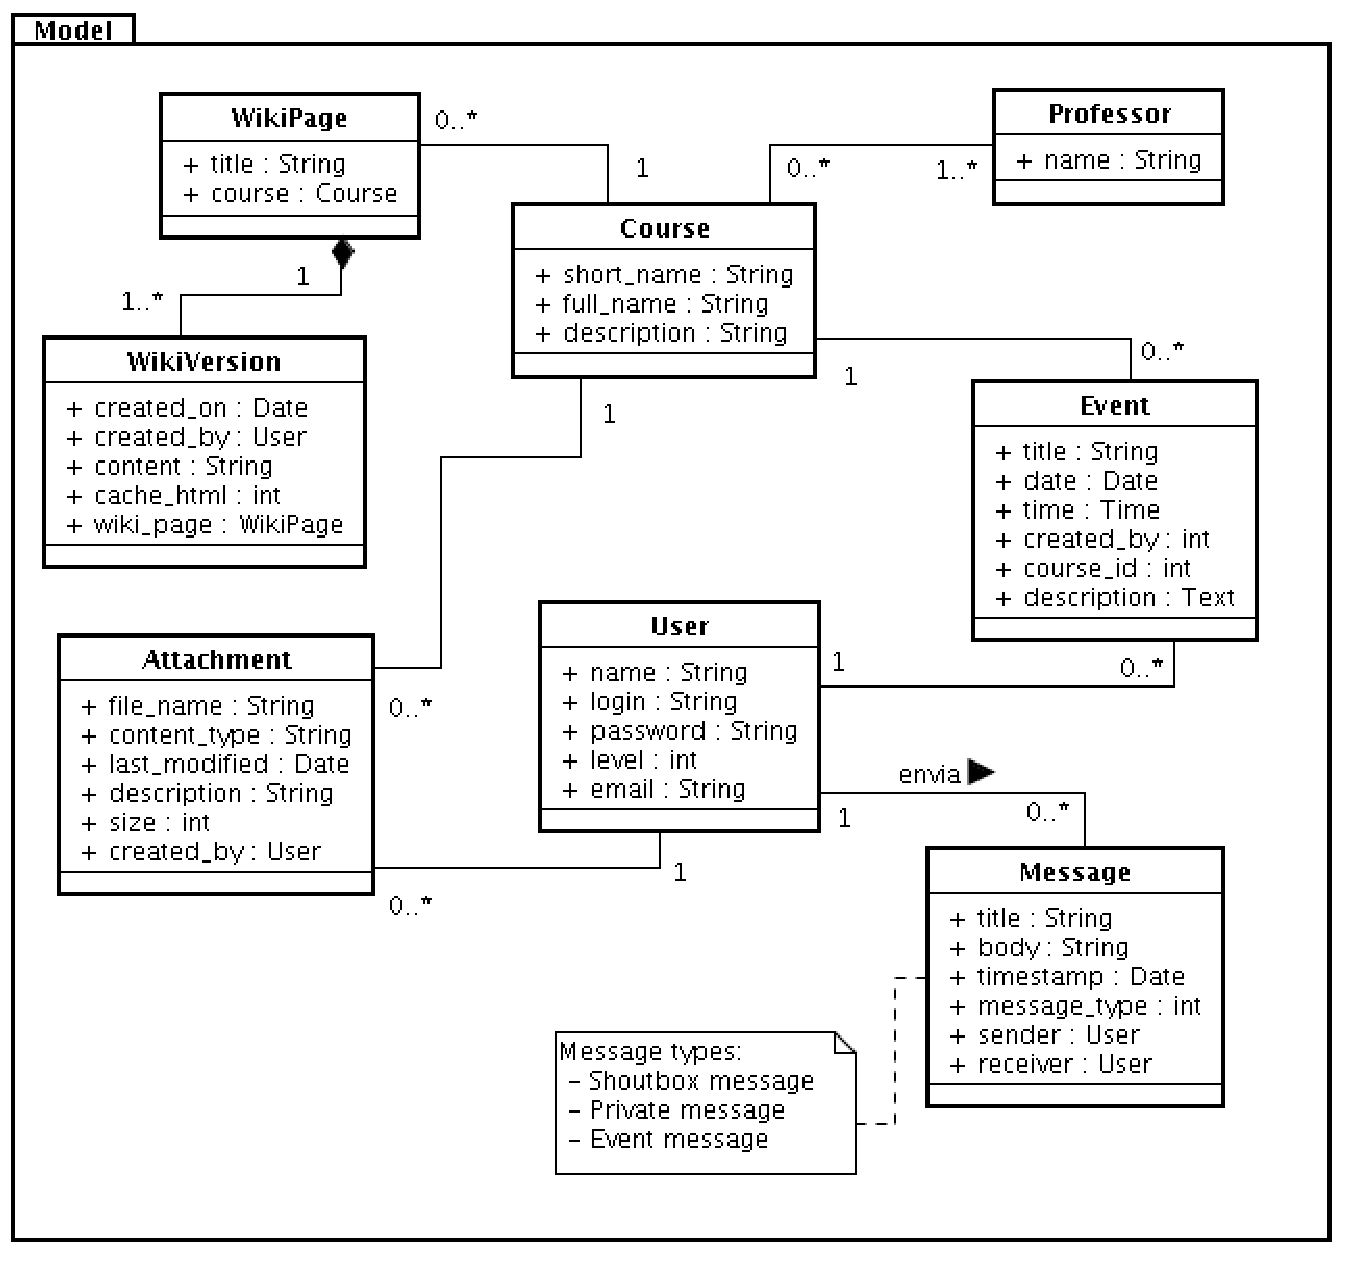
\includegraphics[width=150truemm]{classes-model.pdf}


\pagebreak

% ==========
% Controller
% ==========
\section{Classes Controller}

Cada controller, no Ruby on Rails, implementa um conjunto de ações. Por padrão, essas ações são:

\begin{description}
	\item[index] Indica a página principal do Controller
	\item[list] Exibe todos os elementos cadastrados
	\item[show] Mostra os detalhes de um dos elementos
	\item[new] Mostra o formulário para a criação de um novo objeto
	\item[create] Insere o objeto no banco de dados
	\item[edit] Mostra o formulário para a edição de um objeto
	\item[update] Atualiza o objeto no banco de dados
	\item[destroy] Deleta um elemento do Model
\end{description}

Para simplificação, os métodos CRUD mencionados acima não serão repetidos para as classes a
seguir, uma vez que possuem comportamento semelhante.

\subsection{UserController}

Controller responsável por gerenciar os usuários. Isso inclui fazer logon e logoff, cadastrar novas
contas, alterar preferências e ressetar senhas, caso necessário.

\begin{description}
	\item[signup] Método pelo qual o usuário irá se cadastrar no sistema
	\item[login] Método pelo qual o usuário irá se autenticar no sistema
	\item[logout] Método pelo qual o usuário irá encerrar sua sessão
	\item[forgot\_password] Método a ser utilizado caso o usuário tenha perdido sua senha, enviando uma nova por email
\end{description}

\subsection{MessageController}

Controller responsável pelo envio de mensagens. Usa a estrutura padrão de Controller do Rails.

\subsection{WikiController}

Controller responsável pelas operações sobre o wiki, que incluem edição, criação de novas páginas e
consulta de históricos.

\subsection{CoursesController}

Controller responsável pelo gerenciamento de disciplina. Usa a estrutura padrão de Controller do
Rails.

\subsection{EventsController}

Controller responsável pelo manutenção de eventos no calendário. Usa a estrutura padrão de
Controller do Rails.

\subsection{AttachmentsController}

Controller responsável pelo gerenciamento de arquivos anexos a páginas. Usa a estrutura padrão de
Controller do Rails.

\subsection{Diagrama de Controller}

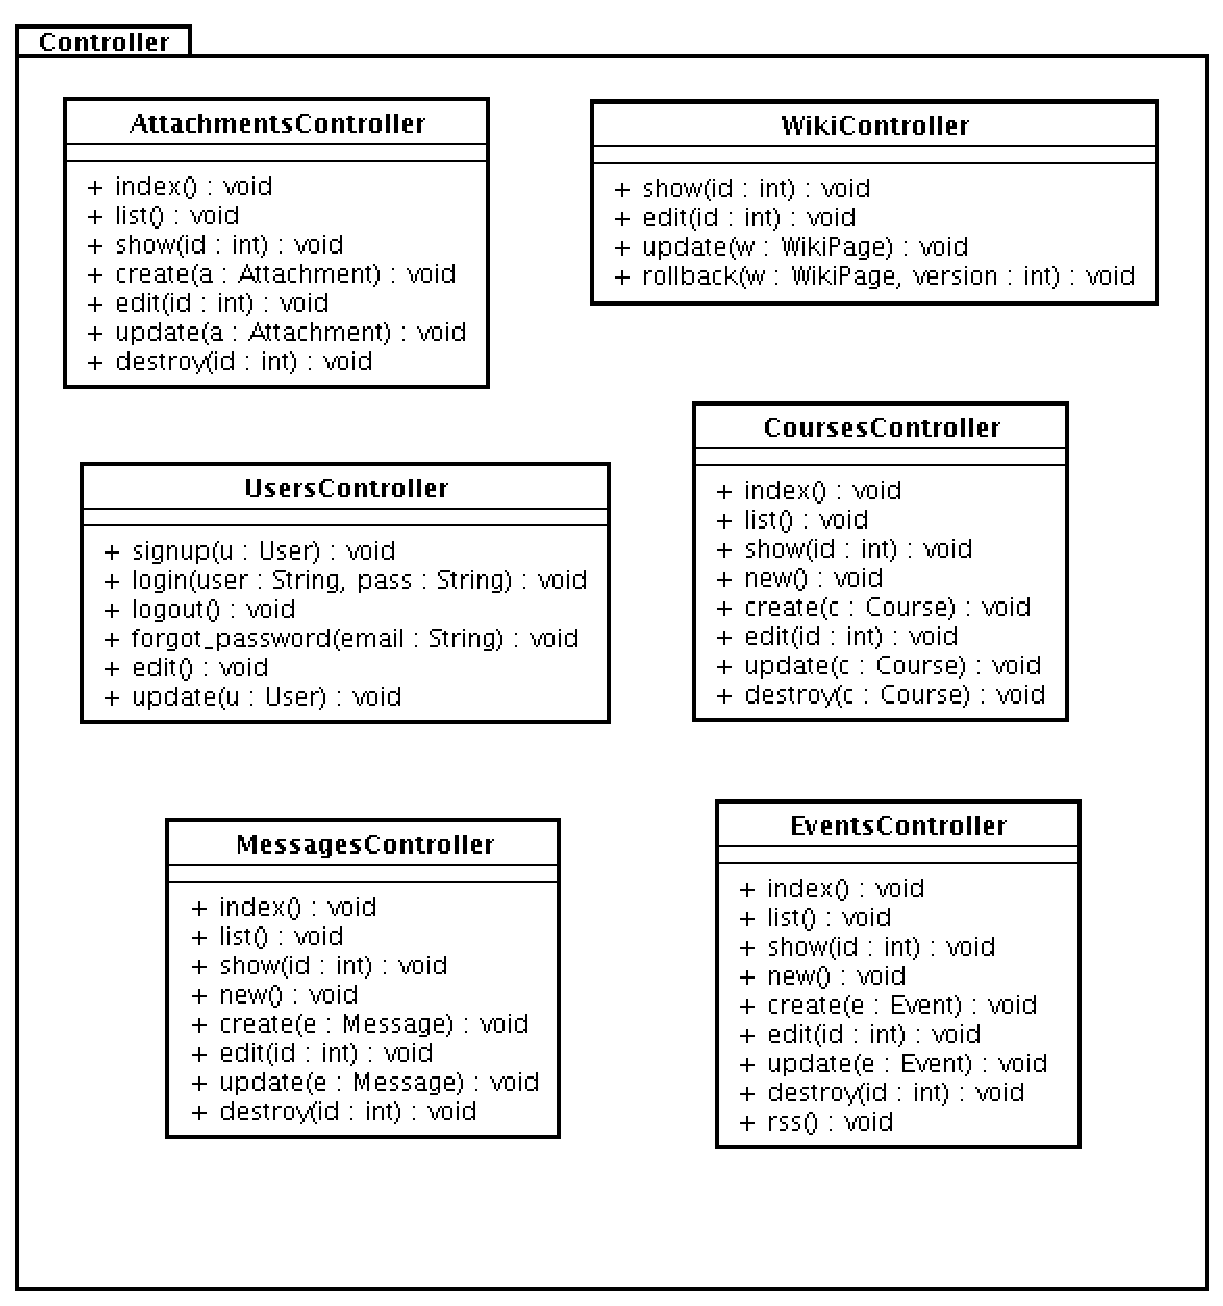
\includegraphics[width=150truemm]{classes-controller.pdf}


\pagebreak

% =====================
% Diagrama de Seqüencia
% =====================

\section{Diagramas de Seqüência}

\subsection{User}
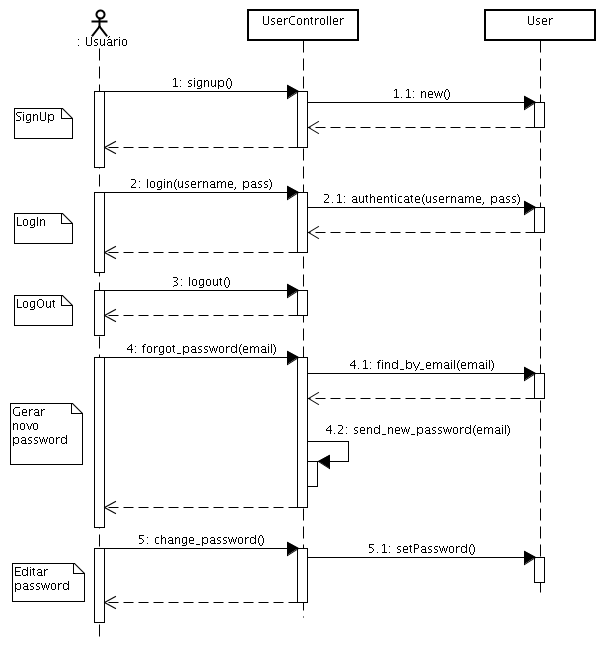
\includegraphics[width=150truemm]{seq_user.png}

\subsection{Attachment}
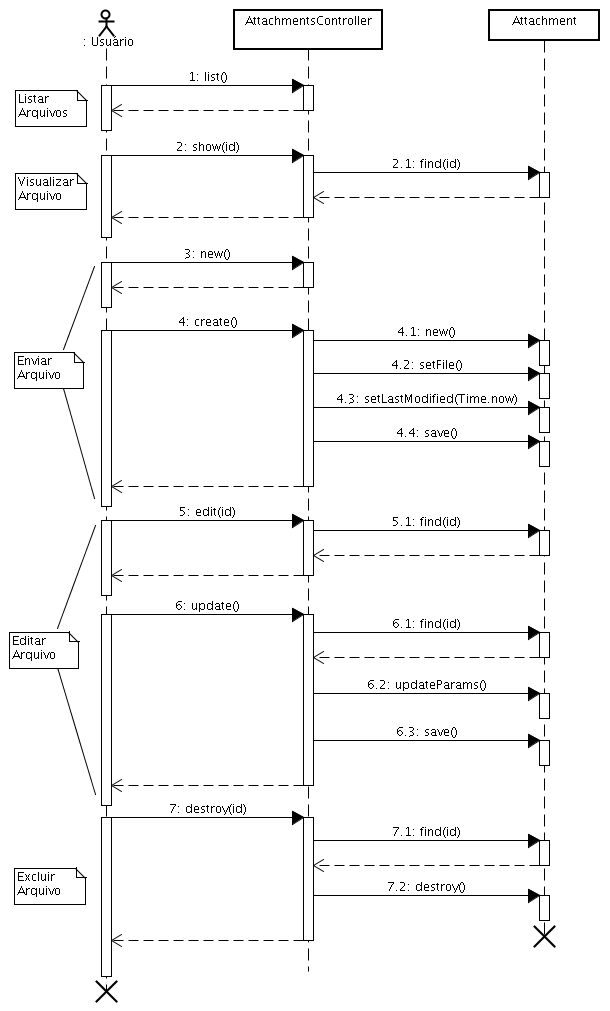
\includegraphics[width=130truemm]{seq_attachment.png}

\subsection{Message}
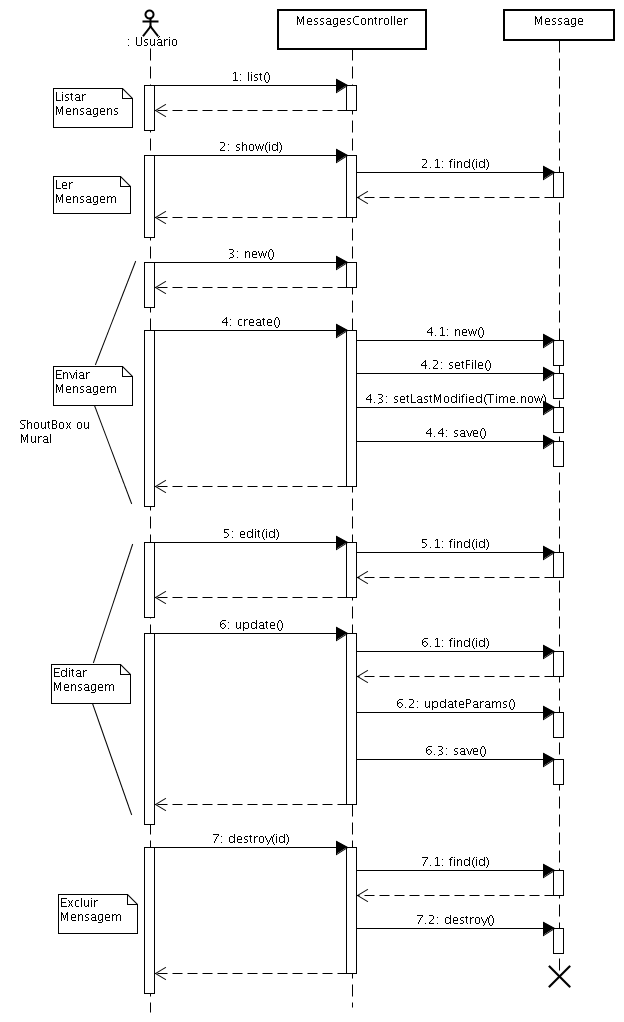
\includegraphics[width=130truemm]{seq_message.png}

\subsection{Course}
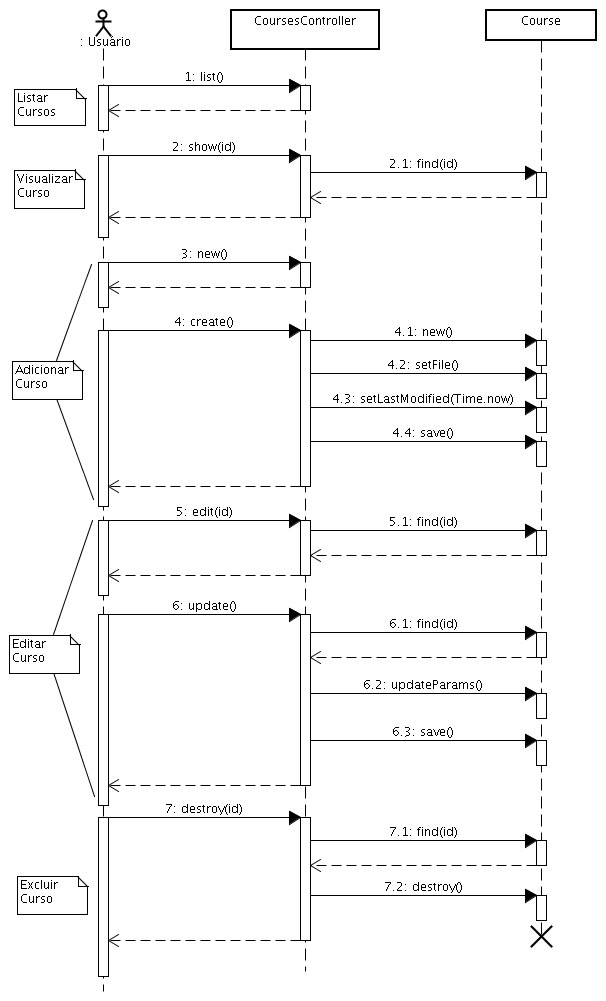
\includegraphics[width=130truemm]{seq_course.png}

\subsection{Event}
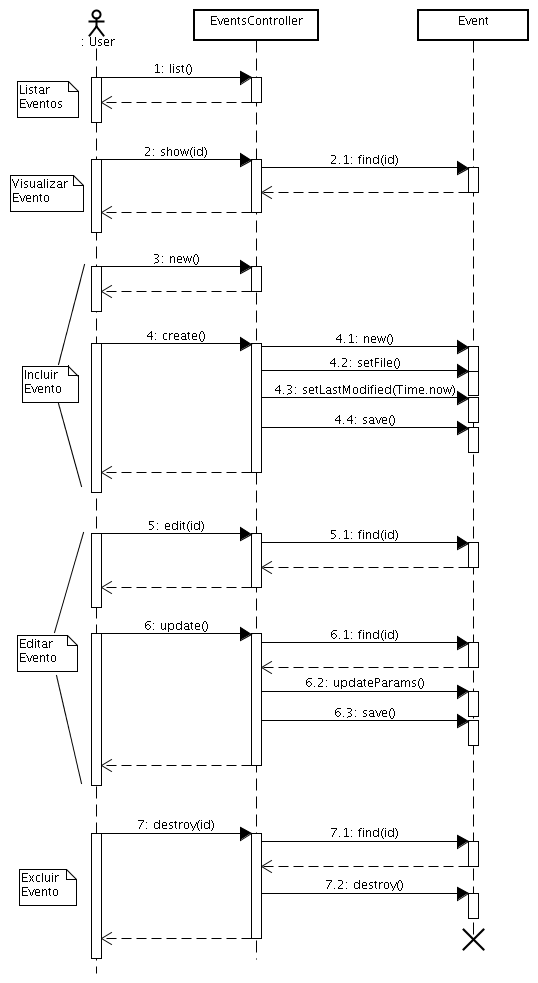
\includegraphics[width=130truemm]{seq_event.png}

\subsection{Wiki}
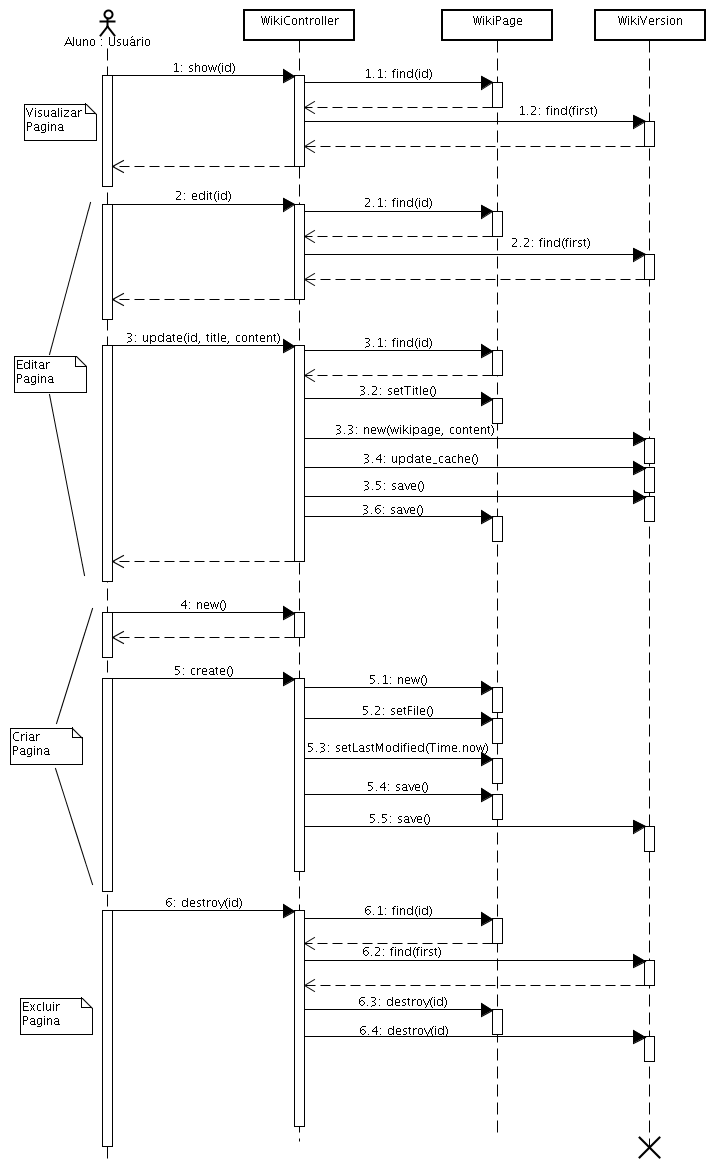
\includegraphics[width=150truemm]{seq_wiki.png}


\end{document}
